\documentclass[10pt]{article}
\usepackage[margin=0.5in]{geometry}
\usepackage{multicol}
\usepackage{lipsum}% dummy text
\usepackage{amsmath}
\usepackage[compact]{titlesec}
\usepackage{graphicx}

\setlength{\columnseprule}{0pt}
\setlength{\parskip}{0pt}
\setlength{\parindent}{0pt} 
\setlength\abovedisplayskip{0pt}
\setlength\belowdisplayskip{0pt}
\setlength{\jot}{0pt}
\linespread{0.9}

\allowdisplaybreaks

\begin{document}
\begin{multicols}{3}

    \section*{Test 1}
    \subsection*{asdfasd}
    asdfasdfasdf
    \subsection*{asdfasd}
    asdfasdfasdf
    \subsection*{asdfasd}
    asdfasdfasdf

    \section*{Test 2}
    \subsection*{asdfasd}
    asdfasdfasdf
    \subsection*{asdfasd}
    asdfasdfasdf
    \subsection*{asdfasd}
    asdfasdfasdf

    \section*{General}
    \subsection*{Demorgans Law}
    \begin{align}
        \neg[p\wedge q]\equiv\neg p\vee\neg q,\\
        \neg[p\vee q]\equiv\neg p\wedge\neg q.
    \end{align}

    \subsection*{Gates}
    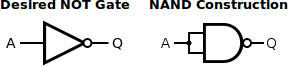
\includegraphics[width=\linewidth]{not.png}
    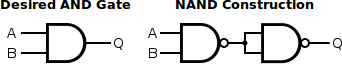
\includegraphics[width=\linewidth]{and.png}
    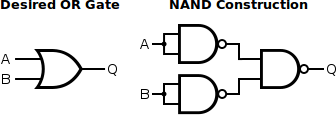
\includegraphics[width=\linewidth]{or.png}
    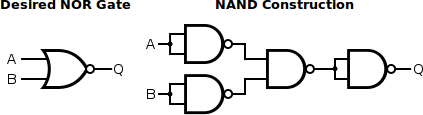
\includegraphics[width=\linewidth]{nor.png}
    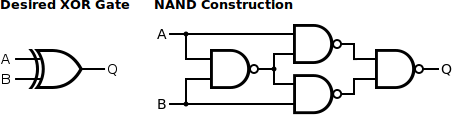
\includegraphics[width=\linewidth]{xor.png}


\end{multicols}
\end{document}
